% !TEX encoding = UTF-8 Unicode
\documentclass[a4paper]{article}

\usepackage{lipsum}
\usepackage{tcolorbox}
\usepackage{color}
\usepackage{url}
%\usepackage[T2A]{fontenc} % enable Cyrillic fonts
\usepackage[utf8]{inputenc} % make weird characters work
\usepackage{graphicx}
\usepackage{amsmath}
%\usepackage[obeyspaces]{url}
\usepackage[T1]{fontenc}
% \usepackage{inconsolata}

\usepackage[english,serbian]{babel}
%\usepackage[english,serbianc]{babel} %ukljuciti babel sa ovim opcijama, umesto gornjim, ukoliko se koristi cirilica

\usepackage[german=quotes]{csquotes}
\DeclareQuoteAlias{ngerman}{serbian}
\MakeOuterQuote{"}

\usepackage[unicode]{hyperref}
\hypersetup{colorlinks,citecolor=green,filecolor=green,linkcolor=blue,urlcolor=blue}

\usepackage{epigraph}

\usepackage{listings}

%\newtheorem{primer}{Пример}[section] %ćirilični primer
\newtheorem{primer}{Primer}[section]

\definecolor{mygreen}{rgb}{0,0.6,0}
\definecolor{mygray}{rgb}{0.5,0.5,0.5}
\definecolor{mymauve}{rgb}{0.58,0,0.82}


\lstset{ 
  backgroundcolor=\color{white},   % choose the background color; you must add \usepackage{color} or \usepackage{xcolor}; should come as last argument
  basicstyle=\scriptsize\ttfamily,        % the size of the fonts that are used for the code
  breakatwhitespace=false,         % sets if automatic breaks should only happen at whitespace
  breaklines=true,                 % sets automatic line breaking
  captionpos=b,                    % sets the caption-position to bottom
  commentstyle=\color{mygreen},    % comment style
  deletekeywords={...},            % if you want to delete keywords from the given language
  escapeinside={\%*}{*)},          % if you want to add LaTeX within your code
  extendedchars=true,              % lets you use non-ASCII characters; for 8-bits encodings only, does not work with UTF-8
  firstnumber=1000,                % start line enumeration with line 1000
  frame=single,	                   % adds a frame around the code
  keepspaces=true,                 % keeps spaces in text, useful for keeping indentation of code (possibly needs columns=flexible)
  keywordstyle=\color{blue},       % keyword style
  language=Python,                 % the language of the code
  morekeywords={*,...},            % if you want to add more keywords to the set
  numbers=left,                    % where to put the line-numbers; possible values are (none, left, right)
  numbersep=5pt,                   % how far the line-numbers are from the code
  numberstyle=\tiny\color{mygray}, % the style that is used for the line-numbers
  rulecolor=\color{black},         % if not set, the frame-color may be changed on line-breaks within not-black text (e.g. comments (green here))
  showspaces=false,                % show spaces everywhere adding particular underscores; it overrides 'showstringspaces'
  showstringspaces=false,          % underline spaces within strings only
  showtabs=false,                  % show tabs within strings adding particular underscores
  stepnumber=2,                    % the step between two line-numbers. If it's 1, each line will be numbered
  stringstyle=\color{mymauve},     % string literal style
  tabsize=2,	                   % sets default tabsize to 2 spaces
  title=\lstname                   % show the filename of files included with \lstinputlisting; also try caption instead of title
}

\begin{document}

\title{Obrada spam mail-ova metodom klasifikacije\\ \small{Seminarski rad u okviru kursa\\Istraživanje podataka\\ Matematički fakultet, Univerzitet u Beogradu}}

\author{Tijana Todorov\\485/2018\\\small{tijana.todorov710@gmail.com}}

\date{19.08.2019}

\maketitle

\abstract{
Cilj ovog rada je da se odredi najbolji spam filter za dobro odvajanje spam mailova od drugih. Ovo je testirano i obrađeno u programskom jeziku Python i IBM-ovom alatu SPSS Modeler pomoću nekoliko metoda koje su obrađene na predavanjima i vežbama.
}

\tableofcontents

\newpage


\section{Uvod}
\label{sec:Uvod}

Spam poruke su zapravo neželjena pošta koja primaocu samo zatrpava sanduče. Ona može biti poruka koja sadrži nešto što primaoca ne zanima, da predstavlja reklamu, online prodavnicu i razne druge stvari. Isto tako ove poruke mogu predstavljati opasnost za primaoca ukoliko su zaražene virusom pa je zato najbolje takve poruke obrisati bez otvaranja. Zbog velikog broja neželjenih poruka koje se iz dana u dan sve više šalju iz raznih razloga kao što je jednostavniji i jeftiniji marketing  vrlo često se dešava da poruke koje primalac očekuje završe greškom u Spam folderu. Iz tog razloga kako bi se što bolje napravila razlika između neželjene pošte i očekivane pošte veoma je bitno napraviti dobar spam filter koji će to razvrstavati. 

\section{Upoznavanje sa podacima}
\label{sec:Upoznavanje}

Podaci koji su korišćeni u ovom  istraživanju se mogu pronaći na \url{https://web.stanford.edu/~hastie/CASI_files/DATA/SPAM.html} pod nazivom \textbf{SPAM.csv}. Skup sadrži podatke o spam porukama. U skupu se nalazi 4601 email poruka upućene istom korisniku sa 59 različitih atributa. Korisnik je označio 1813 email poruka od pristiglih kao spam.


U tabeli ima 57 numeričkih atributa koji predstavljaju najčešće korišćene reči u email porukama koje nisu trivijalne. Za svaku poruku predstavljena je frekvencija tih reči u njoj(procenat pojavljivanja). Osim njih postoje još 2 kategorička
binarna atributa \textbf{spam} i \textbf{testid}.

\begin{itemize}
    \item \textbf{spam} - označava da li je pošta neželjena ili ne
    \item \textbf{testid} - označava da li se instanca nalazi u trening ili test skupu
    \item 48 atributa koji predstavljaju u kom procentu se ta reč pojavljuje u email poruci, po formuli:
\textbf{ 100*broj\_pojavljivanja\_reči / ukupan\_broj\_reči}
(Za reč se smatra da sadrži niz alfanumeričkih karaktera)
	\item 6 atributa (oblika: ch; , ch( , ch[ , ch! , ch\$ , ch\# ) koji predstavljaju u kom procentu se taj karakter nalazi u email poruci, po formuli:
\textbf{ 100*broj\_pojavljivanja\_karaktera / ukupan\_broj\_karaktera}
	\item crl.ave označava prosečnu dužinu neprekidnih nizova velikih slova.
	\item crl.long označava dužinu najduže sekvence velikih slova.
	\item crl.tot označava zbir dužina neprekidnih sekvenci velikih slova tj. ukupan broj velikih slova u email poruci.   
\end{itemize}.

\section{Priprema podataka za obradu}
\label{sec:preprocesiranje}

Zbog velike razlike u opsezima kod atributa, npr: atribut make je u segmentu
[0 - 4.54], a atribut crl.tot u segmentu [1 - 15841] sve atribute sam normalizovala i svela na isti opseg [0 - 1]. U SPSS-u je to obrađeno pomoću čvora \textbf{\_Norm} koji normalizuje izabrane atribute nad kojima sam vršila testiranje. 

Ovakva normalizacija je obrađena i u Python-u sto je prikazano u Listingu \ref{ObradaPy} pored čega su i atributi \textbf{spam} i \textbf{testid} izmenjeni iz tipa Bool u String zbog modela koji zahtevaju da ciljni atribut bude tipa String.

Ciljni atribut nad kojim vršimo testiranje je atribut \textbf{spam}.

\begin{lstlisting}[caption={Obrada podataka u Python-u},frame=single, label=ObradaPy]
booleandf = df.select_dtypes(include=[bool])
booleanDictionary = {True: "tacno", False: "netacno"}

for column in booleandf:
    df[column] = df[column].map(booleanDictionary)

features1 = df.columns[0]
features5 = df.columns[4]
features9 = df.columns[8]
features10 = df.columns[9]
features12 = df.columns[11]
features16 = df.columns[15]
features17 = df.columns[16]
features19 = df.columns[18]
features26 = df.columns[25]

features = [features5, features9, features10, features12, features16, features17, features19, features26]
x_original = df[features]

x=pd.DataFrame(prep.MinMaxScaler().fit_transform(x_original))
\end{lstlisting} 

\section{Drveta odlučivanja}
\label{sec:drveta}

\subsection{SPSS Modeler}

U nastavku će biti upoređeni rezultati primene algoritama C5.0 i C\&Rt što je prikazano na slici \ref{fig:C5CRt_SPSS}. U čvoru \textit{Partition} se vrši podela na trening i test podatke i validacioni skup uzimajući 70\% podataka.

\begin{figure}[ht]
	\centering
    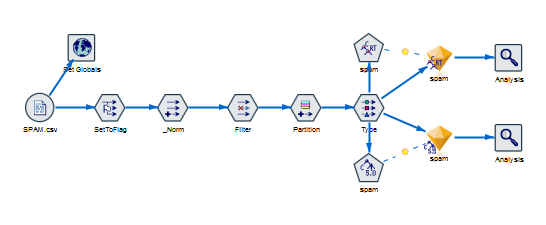
\includegraphics[width=0.8\textwidth]{C5CRt_SPSS.png}
    \caption{Primena modela C5.0 i C\&Rt u SPSS-u}
    \label{fig:C5CRt_SPSS}
\end{figure}


\subsubsection{C5.0}
\label{subsubsec:c50}

Čvor \textit{C5.0} se spaja sa \textit{Type} čvorom gde se nalaze već sređeni podaci. C5.0 metod se poziva sa opcijom Group Symbolics i dobijen rezultat se tumači Analyze čvorom čiji su rezultati prikazani na slikama \ref{fig:C5_grafik} i \ref{fig:C5Tabela}.

\begin{figure}[ht]
	\centering
    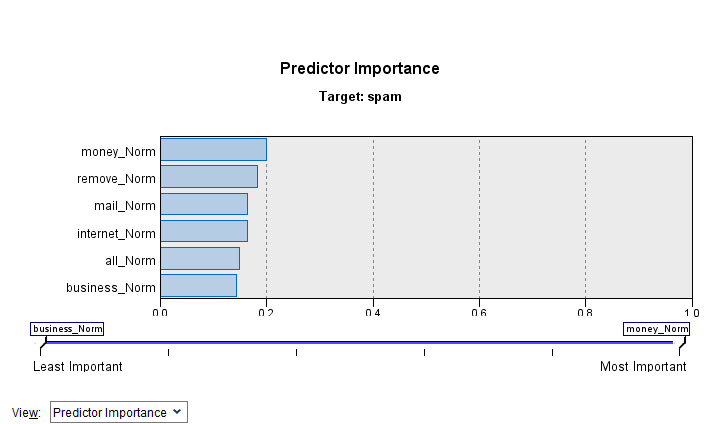
\includegraphics[width=0.6\textwidth]{C5_grafik.png}
    \caption{Bitnost atributa u modelu C5.0}
    \label{fig:C5_grafik}
\end{figure}
            
\begin{figure}[ht]
    \centering
    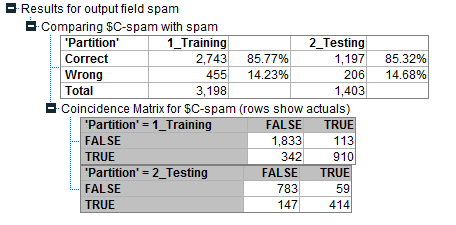
\includegraphics[width=0.6\textwidth]{C5Tabela.png}
    \caption{Rezultat Analyze čvora nad modelom C5.0}
    \label{fig:C5Tabela}
\end{figure}

\subsubsection{C\&RT}
\label{subsubsec:CRT}

Model se pravi pomoću čvora C\&Rt. Cilj je izgraditi novi model u vidu drveta odlučivanja maksimalne dubine 3. Minimalan broj instanci u grani roditelja je 4\%, a u grani deteta 2\%. Kao mera nečistoće koristi se Ginijev kriterijum i minimalnom promenom u nečistoći od 0.0001\%.

Analiza dobijenih rezultata može se videti na slikama \ref{fig:CRtGrafik3} i \ref{fig:CRtTabela3}.

\begin{figure}[ht!]
    \centering
    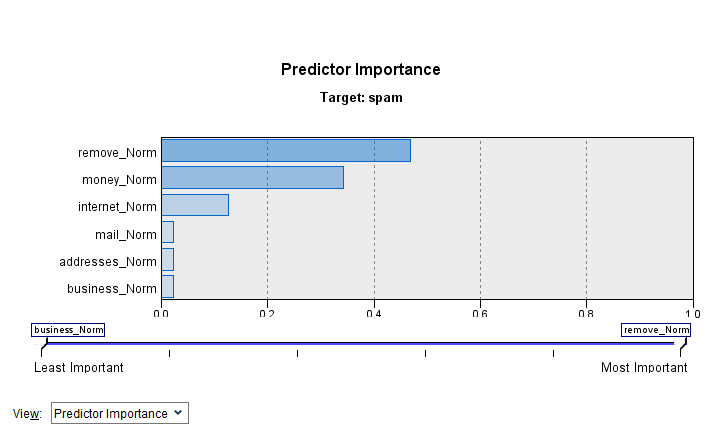
\includegraphics[width=0.6\textwidth]{CRtGrafik3.png}
    \caption{Bitnost atributa u modelu C\&Rt}
    \label{fig:CRtGrafik3}
\end{figure}
        
\begin{figure}[ht!]
    \centering
    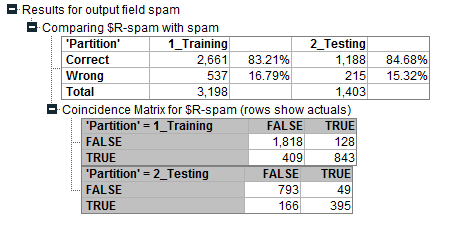
\includegraphics[width=0.6\textwidth]{CRtTabela3.png}
    \caption{Rezultat Analyze čvora nad modelom C\&Rt}
    \label{fig:CRtTabela3}
\end{figure}            
Na slici \ref{fig:CRtStablo2} je prikazano drvo odlučivanja dobijeno generisanjem modela.
\begin{figure}[ht!]
    \centering
    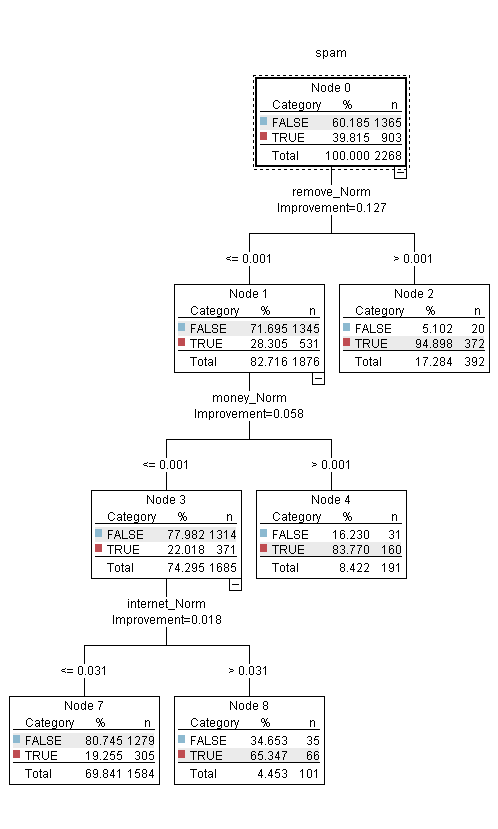
\includegraphics[width=0.7\textwidth]{CRtStablo2.png}
    \caption{Drvo odlučivanja - C\&RT}
    \label{fig:CRtStablo2}
\end{figure}

\subsection{Python}

Primena algoritma drveta odlučivanja u programskom jeziku Python prikazana je u fajlu dtree.py. Podaci se dele u trening i test skup, pri čemu je veličina test skupa 70\% i prethodno je izvršena normalizacija podataka. 


Drvo ima maksimalnu dubinu 12, za kriterijum podele koristi se Ginijev kriterijum i ostvareni su sledeći rezultati za trening i test podatke koji su prikazani u Listingu \ref{TreningTree}:
\\


\begin{lstlisting}[caption={Rezultat nad trening i test podacima},frame=single, label=TreningTree]
#Skup  Trening
Matrica konfuzije
         netacno  tacno
netacno     1882     69
tacno        374    895
Preciznost 0.8624223602484472
Preciznost po klasama [0.83421986 0.92842324]
Odziv po klasama [0.96463352 0.70527975]
Izvestaj klasifikacije
              precision    recall  f1-score   support

     netacno       0.83      0.96      0.89      1951
       tacno       0.93      0.71      0.80      1269

   micro avg       0.86      0.86      0.86      3220
   macro avg       0.88      0.83      0.85      3220
weighted avg       0.87      0.86      0.86      3220

#Skup  Test
Matrica konfuzije
         netacno  tacno
netacno      802     35
tacno        161    383
Preciznost 0.8580738595220855
Preciznost po klasama [0.83281412 0.91626794]
Odziv po klasama [0.95818399 0.70404412]
Izvestaj klasifikacije
              precision    recall  f1-score   support

     netacno       0.83      0.96      0.89       837
       tacno       0.92      0.70      0.80       544

   micro avg       0.86      0.86      0.86      1381
   macro avg       0.87      0.83      0.84      1381
weighted avg       0.87      0.86      0.85      1381
\end{lstlisting} 


\section{Najbliži susedi - KNN}
\label{sec:knn}

\subsection{SPSS Modeler}

U SPSS-u učitavamo podatke, normalizujemo, filtriramo i povezujemo ih sa čvorom \textit{Partition}, koji deli podatke na isti način kao u poglavlju \ref{sec:drveta}. Model se generiše pokretanjem čvora \textit{KNN}, koji prima particionisane podatke kao svoj ulaz. Ciljno polje je označeno kao \textit{spam}, a ostala polja su ulazna. Minimalan broj k je postavljen na 3,  maksimalan na 5, a udaljenost se računa Euklidskim rastojanjem.
Rezultat ovog modela \ref{fig:KNN_SPSS} je prikazan na grafiku \ref{fig:KNNGrafik} i analiziran pomoću čvora Analyze \ref{fig:KNNTabela}.

\begin{figure}[ht!]
    \centering
    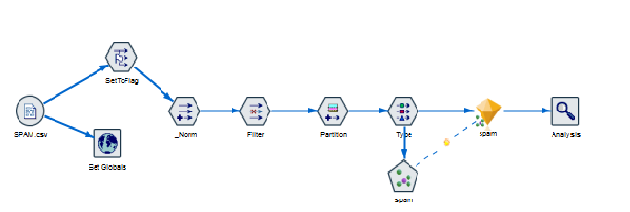
\includegraphics[width=0.8\textwidth]{KNN_SPSS.png}
    \caption{Analiza modela k najbližih suseda - SPSS}
    \label{fig:KNN_SPSS}
\end{figure}
\begin{figure}[ht!]
    \centering
    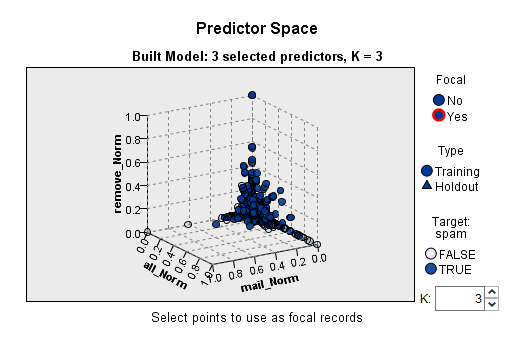
\includegraphics[width=0.6\textwidth]{KNNGrafik.png}
    \caption{Grafikom prikazan rezultat KNN-a u SPSS-u}
    \label{fig:KNNGrafik}
\end{figure}
\begin{figure}[ht!]
	\centering
    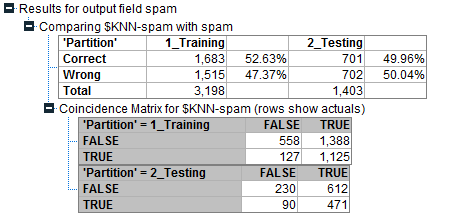
\includegraphics[width=0.6\textwidth]{KNNTabela.png}
    \caption{Rezultat Analyze čvora nad modelom KNN}
    \label{fig:KNNTabela}
\end{figure}            
            
\subsection{Python}

Primena KNN algoritma je opisana u fajlu KNN.py. Veličina trening skupa je postavljena na 70\%. 

Najbolji rezultati dobijaju se za k = 4, Euklidsko rastojanje i kada svi susedi imaju podjednak uticaj, što se vidi na Listingu \ref{KNNpy}.

\begin{lstlisting}[caption={Rezultat KNN-a},frame=single, label=KNNpy]
weights_values = ['uniform', 'distance']
#uniform
Matrica konfuzije
[[793  44]
 [209 335]]

Preciznost 0.8167994207096307
Izvestaj klasifikacije:
              precision    recall  f1-score   support

     netacno       0.79      0.95      0.86       837
       tacno       0.88      0.62      0.73       544

   micro avg       0.82      0.82      0.82      1381
   macro avg       0.84      0.78      0.79      1381
weighted avg       0.83      0.82      0.81      1381

#distance
Matrica konfuzije
[[770  67]
 [163 381]]

Preciznost 0.833454018826937
Izvestaj klasifikacije:
              precision    recall  f1-score   support

     netacno       0.83      0.92      0.87       837
       tacno       0.85      0.70      0.77       544

   micro avg       0.83      0.83      0.83      1381
   macro avg       0.84      0.81      0.82      1381
weighted avg       0.84      0.83      0.83      1381
\end{lstlisting} 

\section{Neuronske mreže}
\label{sec:neuron}

\subsection{SPSS Modeler}

U SPSS-u učitavamo podatke, normalizujemo, filtriramo  i povezujemo ih sa čvorom \textit{Partition}, koji deli podatke na isti način kao u poglavlju \ref{sec:drveta}. Model se generiše pokretanjem čvora \textit{Neural Net}, povezanim sa čvorom \textit{Type}. Za cilj je odabrano kreiranje novog višeslojnog modela.

\begin{figure}[ht!]
	\centering
    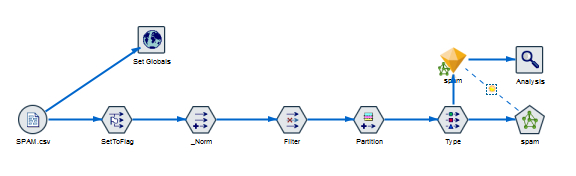
\includegraphics[width=0.8\textwidth]{Neuronske_SPSS.png}
    \caption{Model Neuronske mreže u SPSS-u}
    \label{fig:Neuronske_SPSS}
\end{figure}            


Kreirani model ima 1 skriveni sloj, kao što se vidi na slici \ref{fig:Neuronske4} i razvijao se do trenutka kada više nije bilo moguće smanjiti grešku. Analiza modela prikazana je na slici \ref{fig:Neuronske6}.
\\
\begin{figure}[ht!]
    \centering
    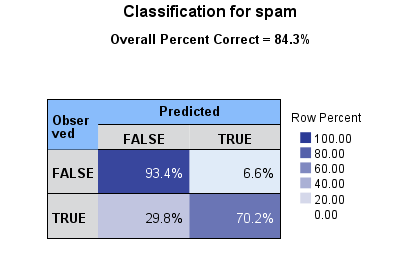
\includegraphics[width=0.7\textwidth]{Neuronske3.png}
    \caption{Matrica konfuzije za neuronske mreže}
    \label{fig:Neuronske3}
\end{figure}

\begin{figure}[ht!]
    \centering
    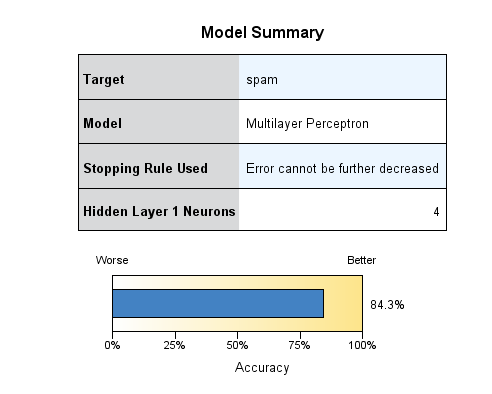
\includegraphics[width=0.4\textwidth]{Neuronske1.png}
    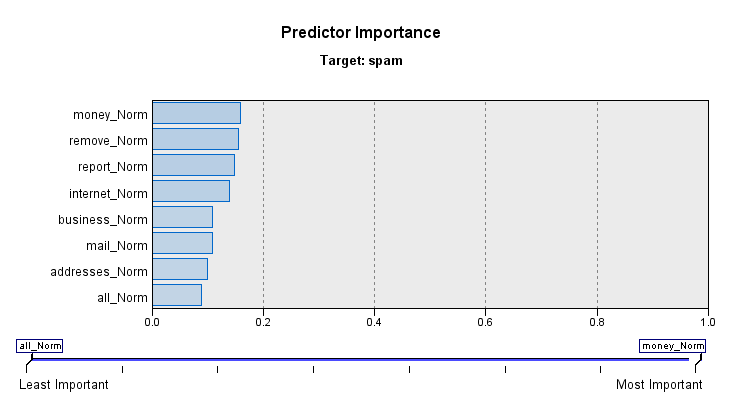
\includegraphics[width=0.4\textwidth]{Neuronske2.png}
    \caption{Neuronska mreža}
    \label{fig:Neuronske1}
\end{figure}


\begin{figure}[ht!]
    \centering
    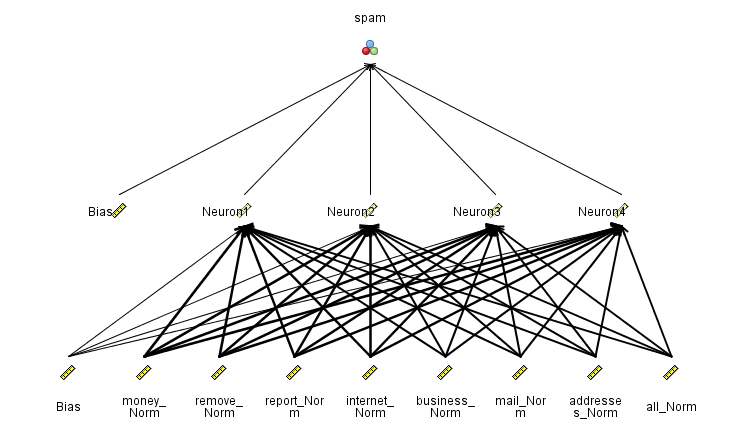
\includegraphics[width=0.9\textwidth]{Neuronske4.png}
    \caption{Neuronska mreža}
    \label{fig:Neuronske4}
\end{figure}
\begin{figure}[ht!]
    \centering
    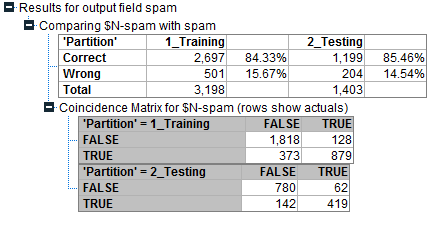
\includegraphics[width=0.7\textwidth]{Neuronske6.png}
    \caption{Rezultat Analyze čvora nad modelom Neuronske mreže}
    \label{fig:Neuronske6}
\end{figure}

\subsection{Python}

Ovaj metod je primenjen na podatke koji su normalizovani kao sto je pomenuto u poglavlju \ref{sec:preprocesiranje}, a opisan je u NeuronskeMLP.py fajlu, čiji je rezultat nad test podacima prikazan u Listingu \ref{NeuronskeTest}. 
\\

\begin{lstlisting}[caption={Rezultat nad test podacima},frame=single, label=NeuronskeTest]
Izvestaj za test skup:
Matrica konfuzije
[[786  51]
 [162 382]]

Preciznost 0.8457639391745112

Izvestaj klasifikacije
              precision    recall  f1-score   support

     netacno       0.83      0.94      0.88       837
       tacno       0.88      0.70      0.78       544

   micro avg       0.85      0.85      0.85      1381
   macro avg       0.86      0.82      0.83      1381
weighted avg       0.85      0.85      0.84      1381

Broj iteracija:  275
Broj slojeva:  4
\end{lstlisting} 


\section{Metod potpornih vektora - SVM}
\label{sec:SVM}

\begin{figure}[ht!]
    \centering
    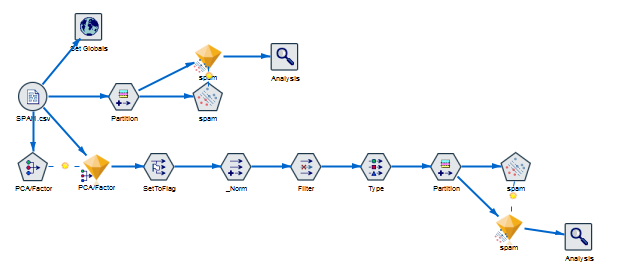
\includegraphics[width=0.8\textwidth]{SVM_SPSS.png}
    \caption{Model SVM u SPSS-u}
    \label{fig:SVM_SPSS}
\end{figure}

Ovaj metod je primenjen u SPSS-u \ref{fig:SVM_SPSS}. Nad učitanim podacima prvo primenjujemo PCA model pomoću PCA čvora kako bismo smanjili skup atributa nad kojim radimo nakon čega ih delimo na trening i test podatke i pokrećemo model SVM pomoću istoimenog čvora. Rezultati dobijeni primenom ovog modela su analizirani pomoću čvora Analyze \ref{fig:SVMTabela} i značajnost atributa su prikazani na \ref{fig:SVMGrafik}. 

\begin{figure}[ht!]
    \centering
    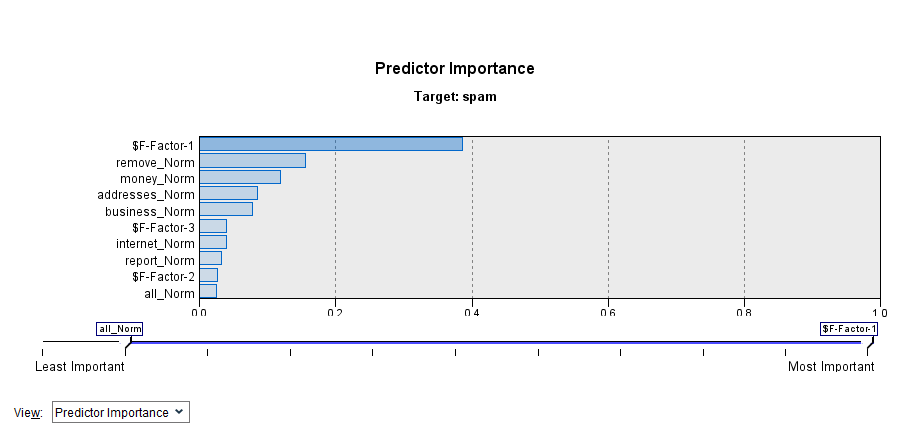
\includegraphics[width=0.6\textwidth]{SVMGrafik.png}
    \caption{Bitnost atributa u modelu SVM}
    \label{fig:SVMGrafik}
\end{figure}
\begin{figure}[ht!]
    \centering
    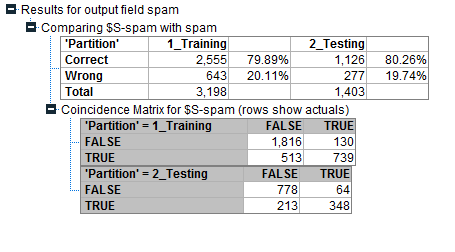
\includegraphics[width=0.6\textwidth]{SVMTabela.png}
    \caption{Rezultat Analyze čvora nad SVM metodom. }
    \label{fig:SVMTabela}
\end{figure}



\section{Gausova klasifikacija}
\label{sec:gaus}

Ovaj metod je primenjen na podatke koji su normalizovani kao sto je pomenuto u poglavlju \ref{sec:preprocesiranje}, a opisan je u Gaus.py fajlu, čiji je jedan deo prikazan u Listingu. Nad podacima je izvršena strafifikacija i za trening skup uzeto je 70\% podataka i rezultat je prikazan u Listingu \ref{Gaus}.

\begin{lstlisting}[caption={Rezultat nad trening podacima},frame=single, label=Gaus]
Matrica konfuzije
[[808  29]
 [306 238]]

Preciznost 0.7574221578566256
Izvestaj klasifikacije
              precision    recall  f1-score   support

       tacno       0.73      0.97      0.83       837
     netacno       0.89      0.44      0.59       544

   micro avg       0.76      0.76      0.76      1381
   macro avg       0.81      0.70      0.71      1381
weighted avg       0.79      0.76      0.73      1381

\end{lstlisting} 


\newpage

\section{Zaključak}
\label{sec:Zakljucak}

Analiziranjem SPAM.csv skupa podataka metodom klasifikacije i primenom sledecih metoda: C5.0, C\&Rt, KNN, Neuronske mreže, SVM i Gausa dolazimo do zaključka da \textbf{C\&Rt} daje najbolje rezultate. Sve ove metode su obrađene u SPSS-u i Python-u ali je njihovo poređenje izvšeno u SPSS-u pomoću čvora \textbf{Auto Classifier} \ref{fig:Poredjenje_SPSS} koji je primenjen nad već obrađenim, normalizovanim podacima. 

\begin{figure}[ht!]
    \centering
    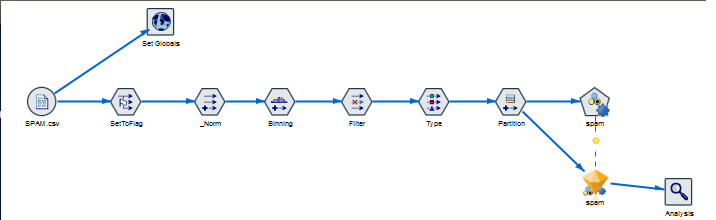
\includegraphics[width=0.9\textwidth]{Poredjenje_SPSS.png}
    \caption{Poređenje svih metoda u SPSS-u}
    \label{fig:Poredjenje_SPSS}
\end{figure}

Pokretanjem \textbf{Auto Classifier} dobijamo za rezultat sledecu tabelu koja je prikazana na slici  \ref{fig:Poredjenje} gde su metodi sortirani od onog koji daje najbolje do onog koji daje najlošije rezultate nad ovim skupom podataka.

\begin{figure}[ht!]
    \centering
    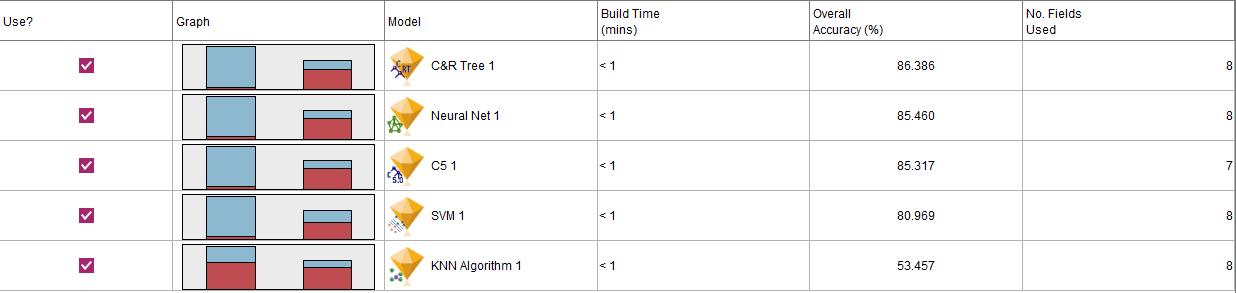
\includegraphics[width=1.2\textwidth]{Poredjenje.png}
    \caption{Rezultat poređenja svih metoda}
    \label{fig:Poredjenje}
\end{figure}

Rezultat dobijen na prethodnoj slici smo analizirali čvorom Analyze koji je vratio sledeci rezultat \ref{fig:PoredjenjeTabela}.

\begin{figure}[ht!]
    \centering
    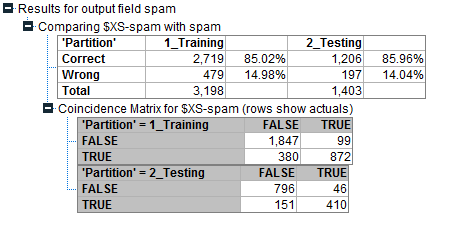
\includegraphics[width=0.6\textwidth]{PoredjenjeTabela.png}
    \caption{Rezultat Analyze čvora nad čvorom koji poredi sve metode}
    \label{fig:PoredjenjeTabela}
\end{figure}

\addcontentsline{toc}{section}{Literatura}
\appendix
\bibliography{literatura} 
\bibliographystyle{plain}

\end{document}